\documentclass{beamer}

\usepackage{graphicx}
\usepackage{amsmath}
\usepackage{float}

% Definição do idioma
\usepackage[brazil]{babel}
\usepackage[utf8]{inputenc}
\usepackage{amsmath}  % Para as equações

% Escolha do tema (opcional)
\usetheme{Hannover}

% Definição do título, autores e data
\title{Predição da Estabilidade de uma Smart Grid}
\author{Victor Jorge  \\ João Vinicius }
\date{\today}

\begin{document}

% Slide de título
\begin{frame}
    \titlepage
\end{frame}

% Sumário
\begin{frame}{Sumário}
    \tableofcontents
\end{frame}

% Slide 1: Smart Grid
\section{Smart Grid}

\begin{frame}{O que é Smart Grid?}

    \begin{itemize}
        \item Rede elétrica inteligente que utiliza tecnologia digital.
        \item Monitora, controla e otimiza produção, distribuição e consumo de energia.
        \item Integra sistemas de comunicação, automação e dados.
        \item Permite gestão eficiente da energia e detecção de falhas.
        \item Facilita a incorporação de fontes de energia renovável.
        \item Incentiva a participação ativa dos consumidores.
    \end{itemize}

\end{frame}

% Slide 2: Motivação do Estudo
\section{Motivação do Estudo}

\begin{frame}{Motivação do Estudo}
    \begin{itemize}
        \item Problemas identificados no gerenciamento de redes elétricas
        \item Necessidade de prever a estabilidade em cenários complexos
        \item Impacto esperado: Melhorar a confiabilidade e eficiência energética
    \end{itemize}
\end{frame}

% Slide 3: Metodologia - Visão Geral
\section{Metodologia}

\begin{frame}{Metodologia - Visão Geral}
    \begin{itemize}
        \item Abordagem de Regressão: Comparação de 18 modelos
        \item Uso de Algoritmo Genético para otimização de parâmetros
        \item Avaliação e escolha dos melhores modelos
    \end{itemize}
\end{frame}

% Slide 4: Regressão - Tipos de Regressão
\begin{frame}{Regressão - Tipos de Regressão}
    \begin{footnotesize}
        \begin{itemize}
            \item {Bayesian Ridge Regression}
            \item {Automatic Relevance Determination (ARD) Regression}
            \item {Lasso Regression}
            \item {Ridge Regression}
            \item {Linear Regression}
            \item {Support Vector Regression (SVR)}
            \item {Nu Support Vector Regression (NuSVR)}
            \item {Light Gradient Boosting Machine (LGBM)}
            \item {k-Nearest Neighbors Regression (KNN)}
            \item {Elastic Net Regression}
            \item {AdaBoost Regression}
            \item {Stochastic Gradient Descent Regression (SGD)}
            \item {Extra Trees Regression}
            \item {eXtreme Gradient Boosting (XGBoost)}
            \item {Multi-layer Perceptron Regression (MLP)}
            \item {Random Forest Regression}
            \item {Histogram-based Gradient Boosting Regression}
            \item {Gradient Boosting Regression}
            \item {Decision Tree Regression}
        \end{itemize}
    \end{footnotesize}
\end{frame}

% Slide 5: Regressão - Nu Support Vector Regression (NuSVR)
\begin{frame}{Regressão - Nu Support Vector Regression (NuSVR)}
    \begin{itemize}
        \item Utiliza o parâmetro Nu como limite superior e inferior
        \item Capacidade de modelar relações complexas em dados de alta dimensionalidade
        \item Resultado: Melhor desempenho em termos de R² e MAPE
    \end{itemize}
\end{frame}

% Slide 6: Regressão - LightGBM
\begin{frame}{Regressão - LightGBM}
    \begin{itemize}
        \item Combina vários modelos individuais de árvores de decisão para regressão
        \item Foco em desempenho e rapidez de treinamento
        \item Resultado: Alta robustez e generalização, com menor tendência ao overfitting
    \end{itemize}
\end{frame}

% Slide 7: Regressão - Histogram-based Gradient Boosting Regression
\begin{frame}{Regressão - Histogram-based Gradient Boosting Regression}
    \begin{itemize}
        \item Similar ao LightGBM, mas usa histogramas para simplificar splits
        \item Melhora a eficiência em grandes conjuntos de dados
        \item Resultado: Boa precisão, mas tendência ao overfitting em alguns casos
    \end{itemize}
\end{frame}

% Slide 8: Algoritmo Genético
\begin{frame}{Algoritmo Genético}
    \begin{itemize}
        \item Estrutura da equação utilizada:
              \[
                  \lambda_1 x_1 + \lambda_2 x_2 + \dots + \lambda_n x_n = Y
              \]
        \item Parâmetros: Número de gerações, mutação, crossover, etc.
        \item Uso da biblioteca \texttt{pygad} para implementação
        \item Desempenho: Melhorias significativas em parâmetros de regressão
    \end{itemize}
\end{frame}

% Slide 9: Resultados e Discussões
\section{Resultados e Discussões}

% Slide 1: Title Slide
\begin{frame}
    \title{Resultados e Discussões}
    \author{}
    \date{}
    \maketitle
\end{frame}

% Slide 2: Mapa de Calor - Correlações
\begin{frame}{Regressão: Mapa de Calor - Correlações}
    \begin{figure}[H]
        \centering
        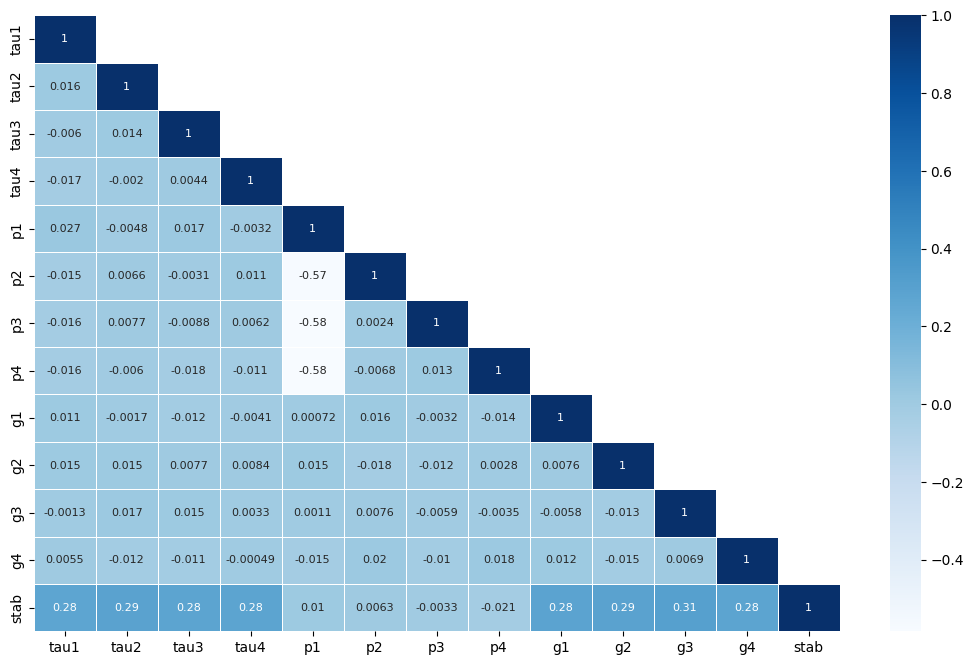
\includegraphics[width=0.9\linewidth]{Mapa_calor_corr.png}
        \caption{Mapa de calor - Correlações}
    \end{figure}

    \begin{itemize}
        \item Algumas variáveis apresentaram correlação fraca, mas relevante.
        \item As variáveis g's tiveram correlação com stab, com uma correlação positiva de aproximadamente 0.54.
    \end{itemize}
\end{frame}

% Slides 3-6: Resultados dos 18 Modelos
\begin{frame}{Resultados: MAE dos 18 Modelos}
    \begin{figure}[H]
        \centering
        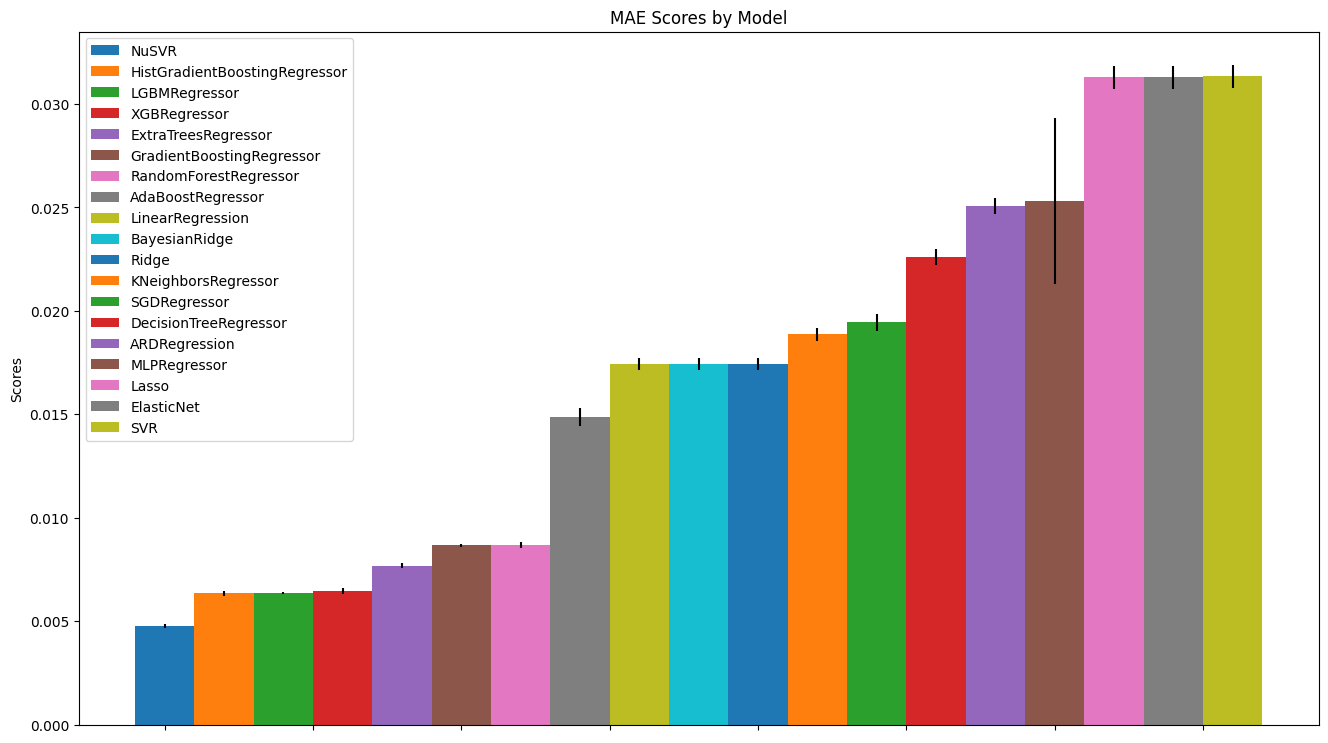
\includegraphics[width=1\linewidth]{image.png}
        \caption{Resultado MAE dos 18 modelos}
    \end{figure}
\end{frame}

\begin{frame}{Resultados: MSE dos 18 Modelos}
    \begin{figure}[H]
        \centering
        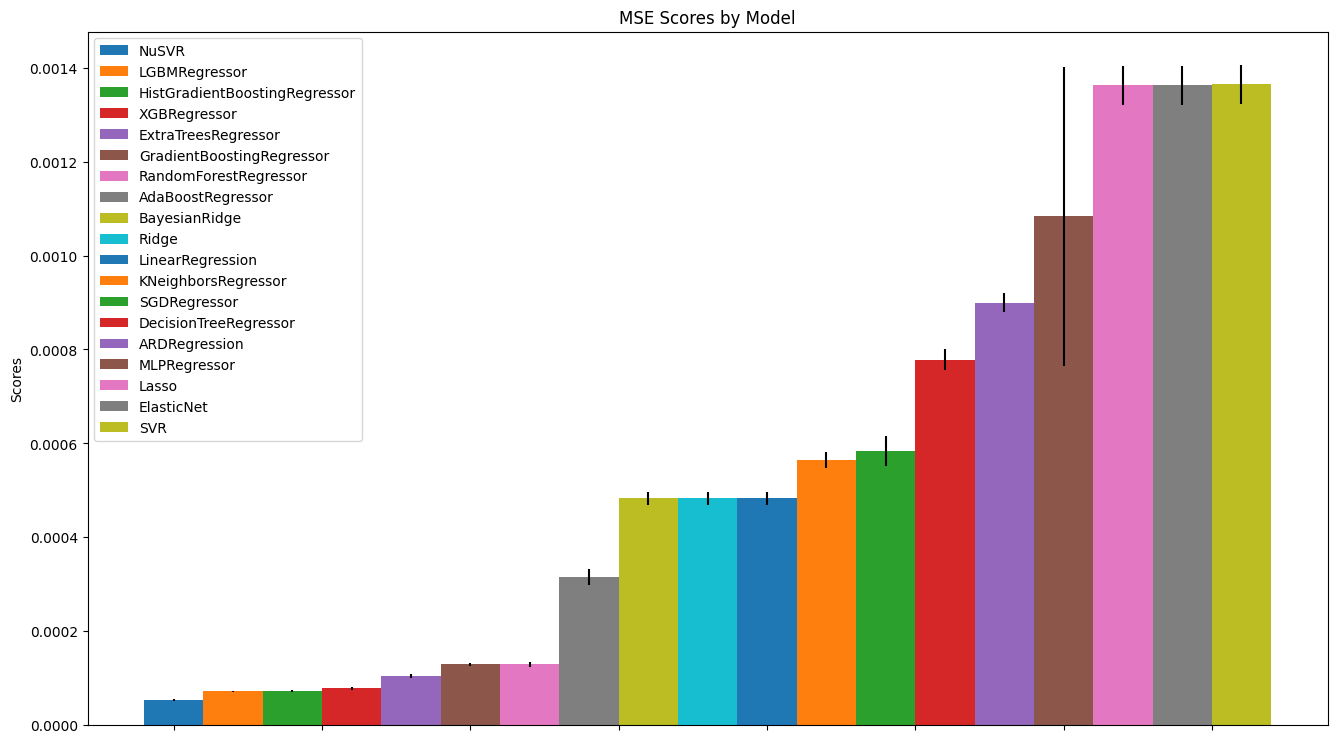
\includegraphics[width=1\linewidth]{image3.png}
        \caption{Resultado MSE dos 18 modelos}
    \end{figure}
\end{frame}

\begin{frame}{Resultados: MAPE dos 18 Modelos}
    \begin{figure}[H]
        \centering
        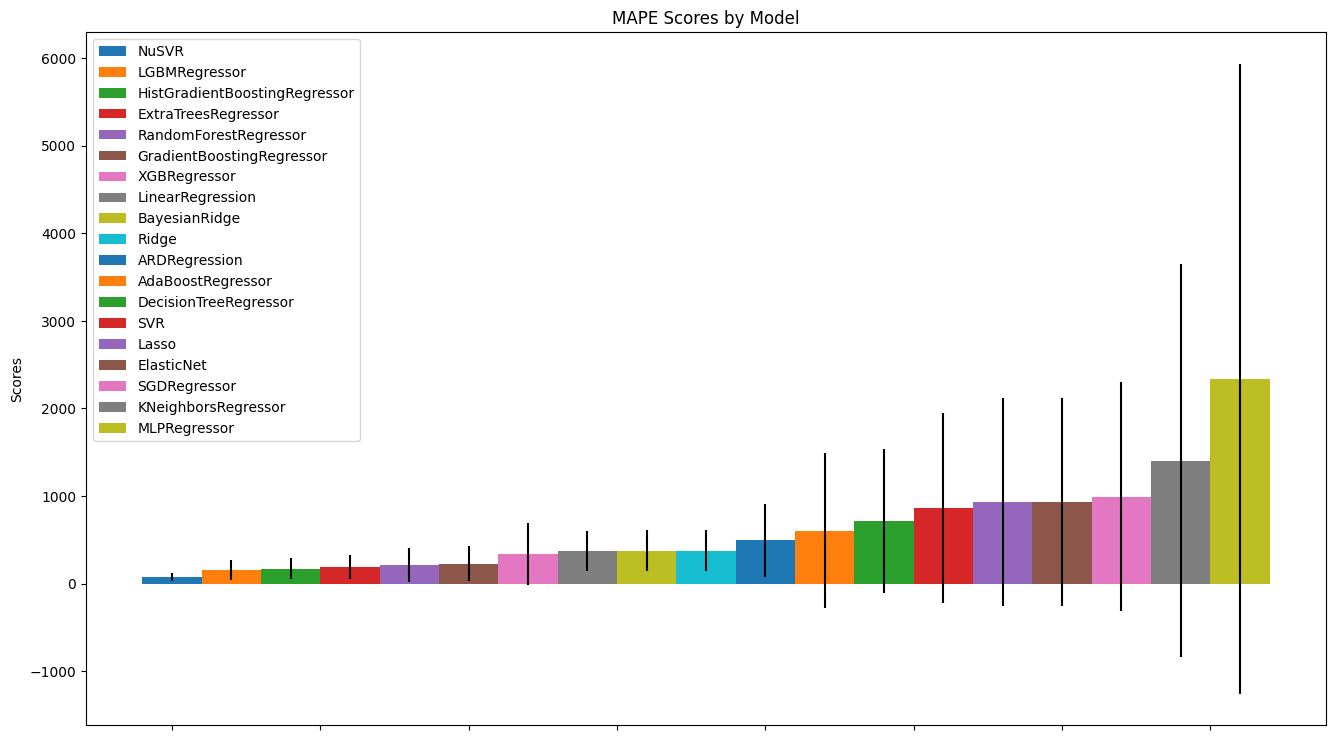
\includegraphics[width=1\linewidth]{image4.png}
        \caption{Resultado MAPE dos 18 modelos}
    \end{figure}
\end{frame}

\begin{frame}{Resultados: R² dos 18 Modelos}
    \begin{figure}[H]
        \centering
        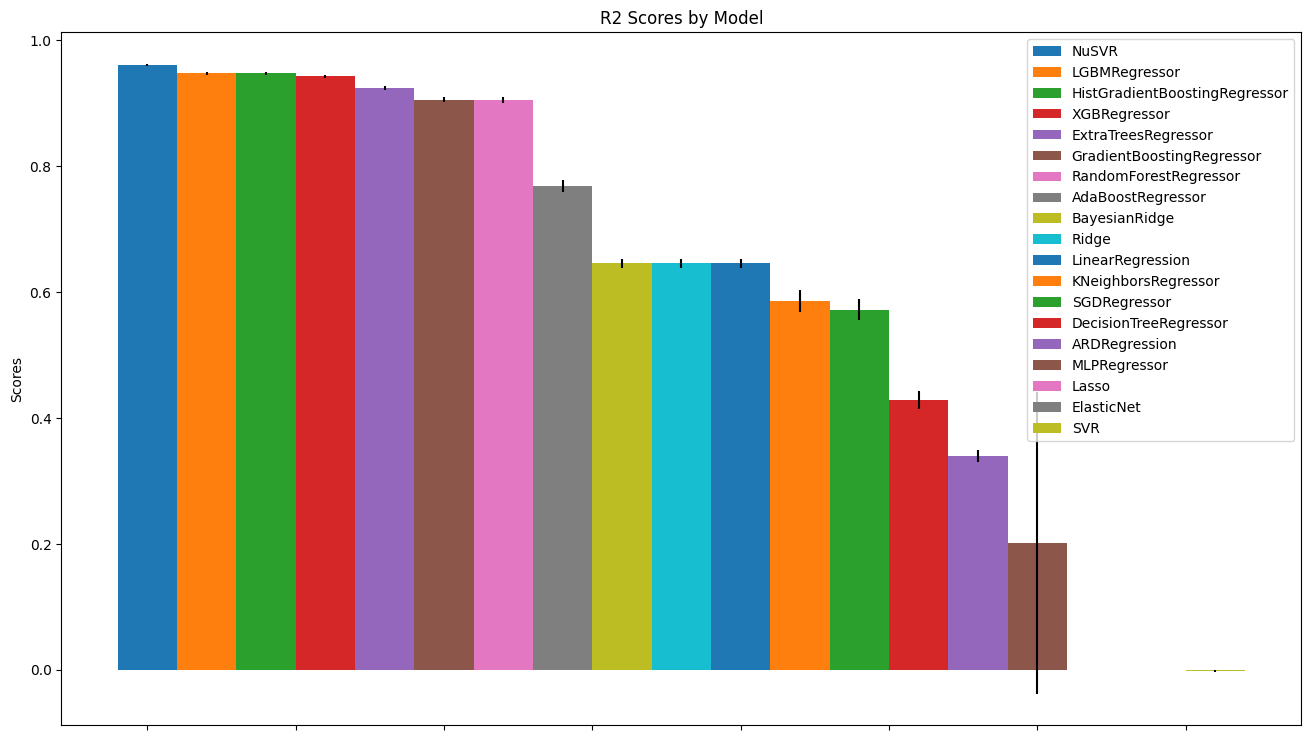
\includegraphics[width=1\linewidth]{image2.png}
        \caption{Resultado R² dos 18 modelos}
    \end{figure}
\end{frame}

% Slide 7: Modelos Performáticos
\begin{frame}{Modelos Performáticos}
    \textbf{Modelos que performaram melhor:}
    \begin{itemize}
        \item NuSVR
        \item LightGBM
        \item HistGradientBoosting
    \end{itemize}
    \textbf{Análise:}
    \begin{itemize}
        \item Aplicado Grid Search para melhorar hiperparâmetros.
        \item Foram analisados MSE, MAPE, MAE e R².
    \end{itemize}
\end{frame}

% Slide 8: MSE dos Modelos Escolhidos
\begin{frame}{MSE dos Modelos Escolhidos}
    \begin{figure}[H]
        \centering
        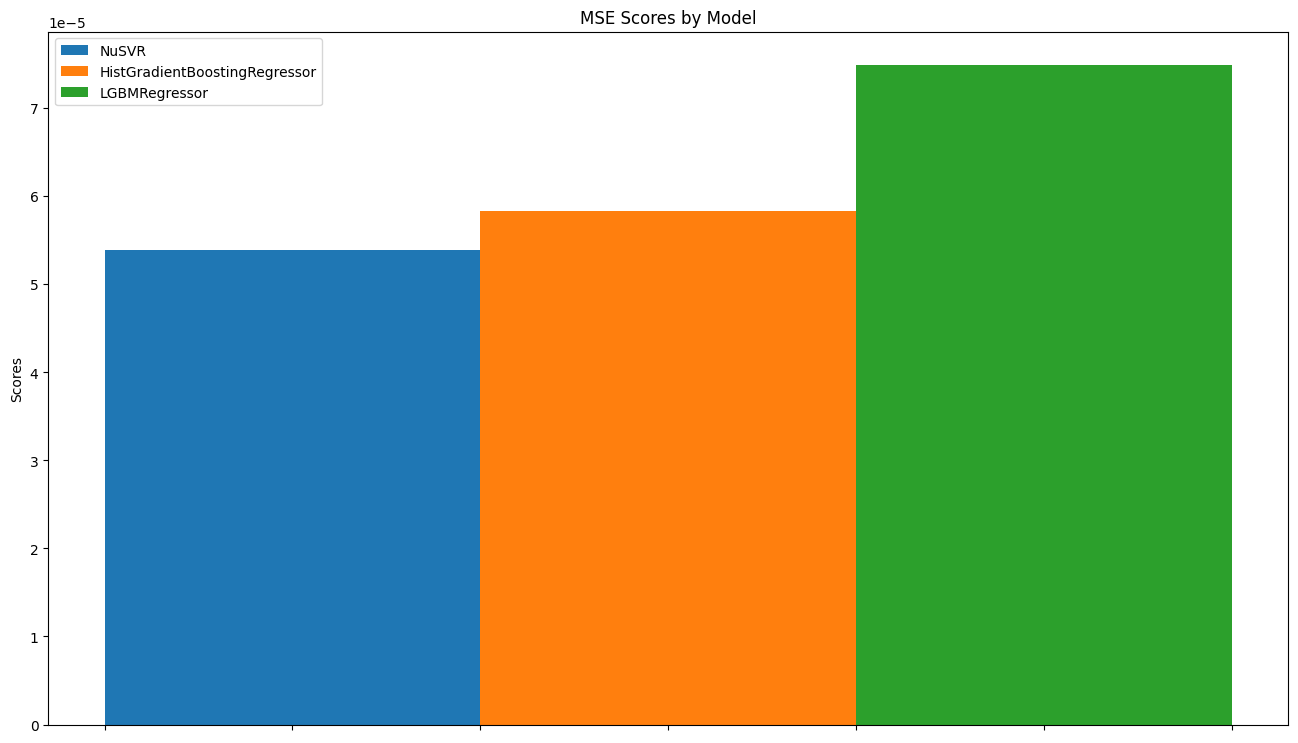
\includegraphics[width=1\linewidth]{7.png}
        \caption{MSE dos Modelos Escolhidos}
    \end{figure}
\end{frame}

% Slide 9: MAPE dos Modelos Escolhidos
\begin{frame}{MAPE dos Modelos Escolhidos}
    \begin{figure}[H]
        \centering
        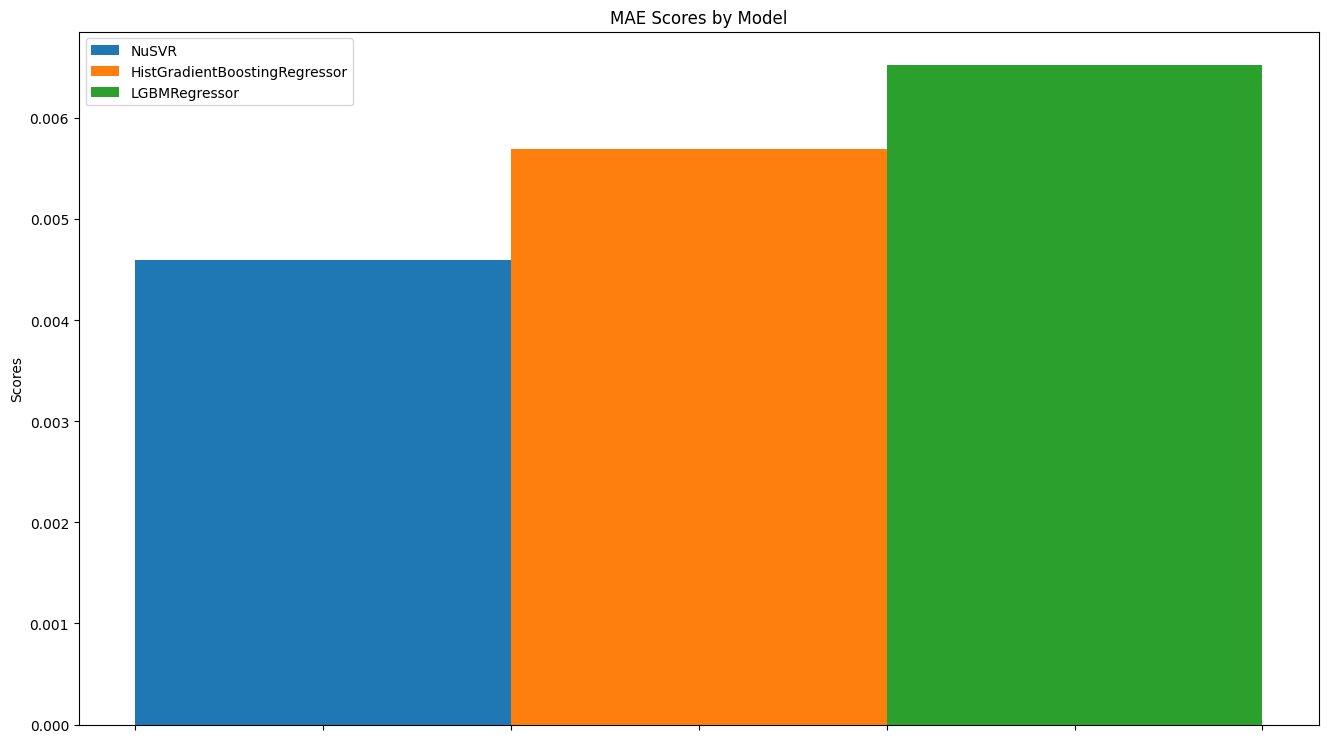
\includegraphics[width=1\linewidth]{9.png}
        \caption{MAPE dos Modelos Escolhidos}
    \end{figure}
\end{frame}

% Slide 10: MAE dos Modelos Escolhidos
\begin{frame}{MAE dos Modelos Escolhidos}
    \begin{figure}[H]
        \centering
        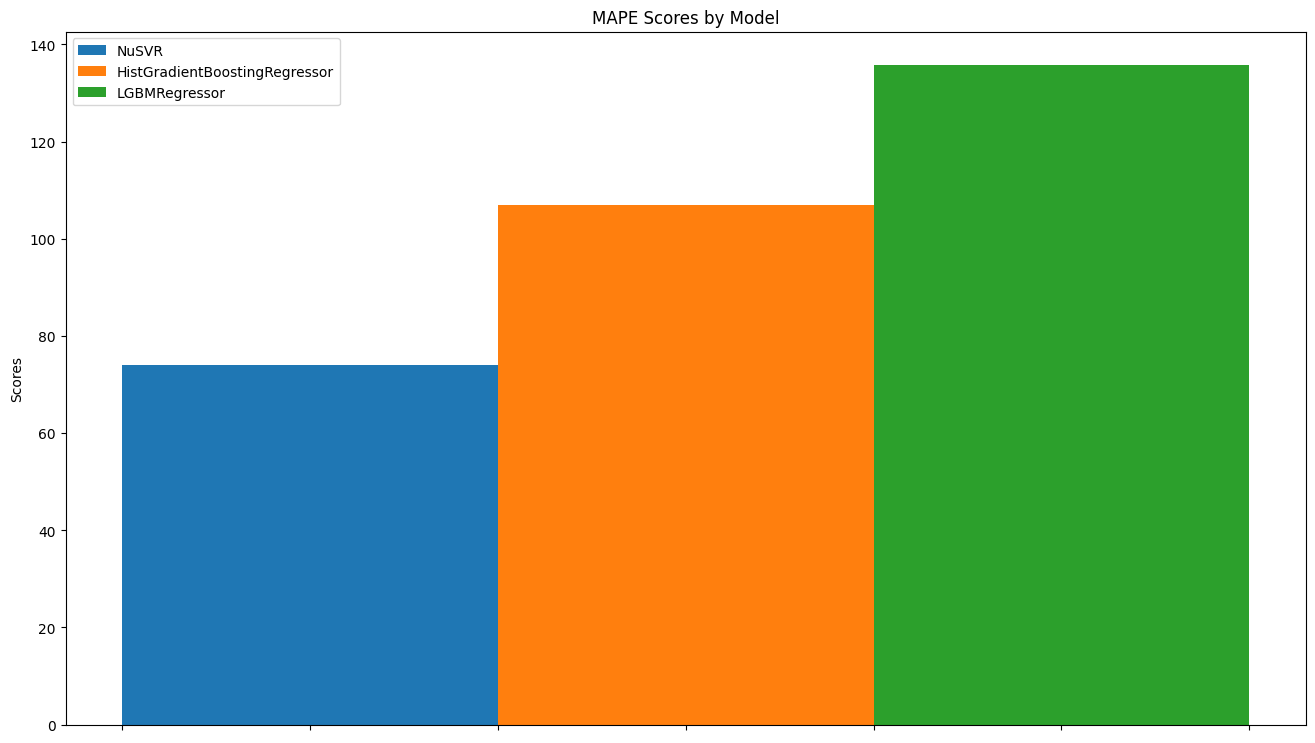
\includegraphics[width=1\linewidth]{10.png}
        \caption{MAE dos Modelos Escolhidos}
    \end{figure}
\end{frame}

% Slide 11: R² dos Modelos Escolhidos
\begin{frame}{R² dos Modelos Escolhidos}
    \begin{figure}[H]
        \centering
        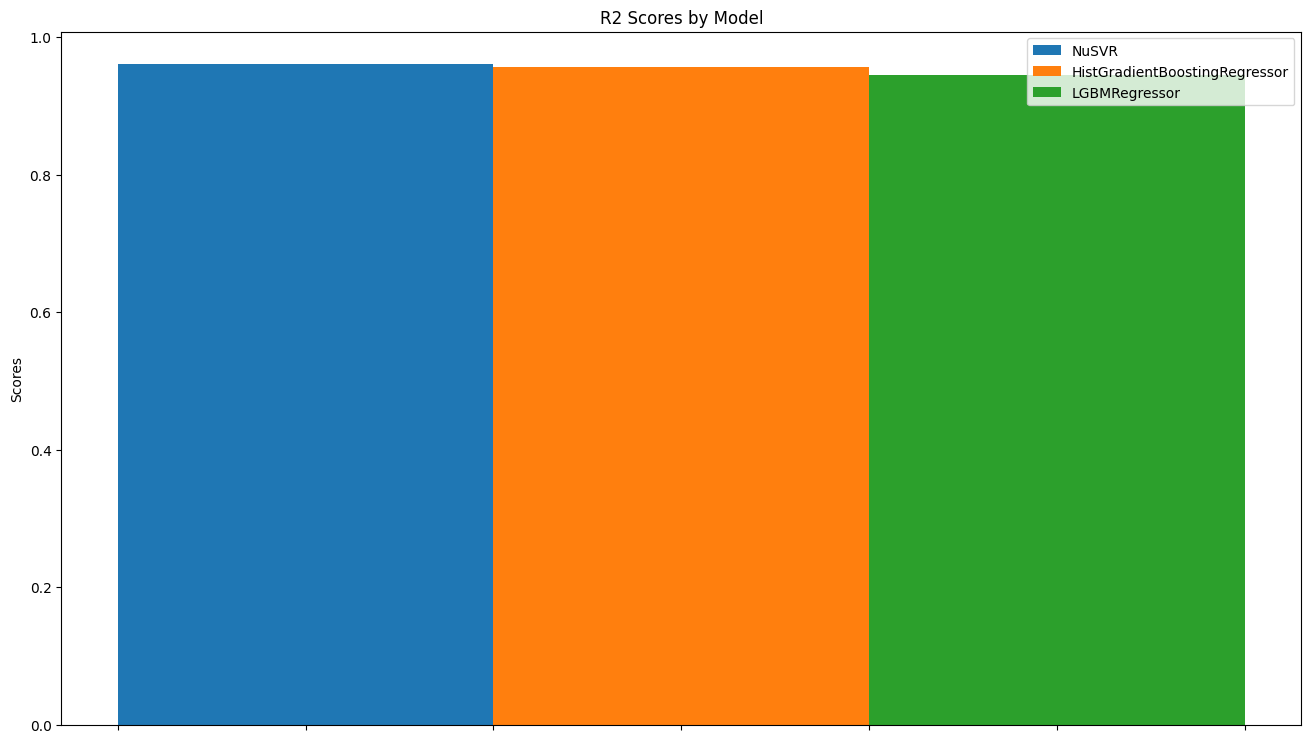
\includegraphics[width=1\linewidth]{12.png}
        \caption{R² dos Modelos Escolhidos}
    \end{figure}
\end{frame}

% Slide 12: Equações dos Modelos Escolhidos
\begin{frame}{Equações dos Modelos Escolhidos}
    \begin{itemize}
        \item Avaliação de funções para utilizar a navalha de Occam.
    \end{itemize}
    \begin{figure}[H]
        \centering
        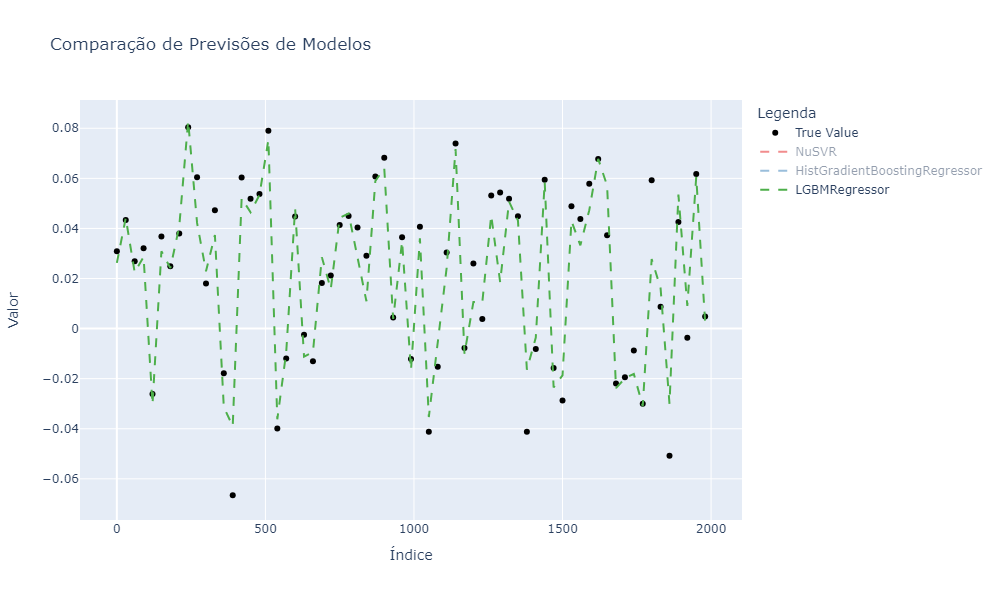
\includegraphics[width=1\linewidth]{LGBMRegressor_func.png}
        \caption{Função da LightGBMRegressor}
    \end{figure}
\end{frame}

\begin{frame}{Função da NuSVR}
    \begin{figure}[H]
        \centering
        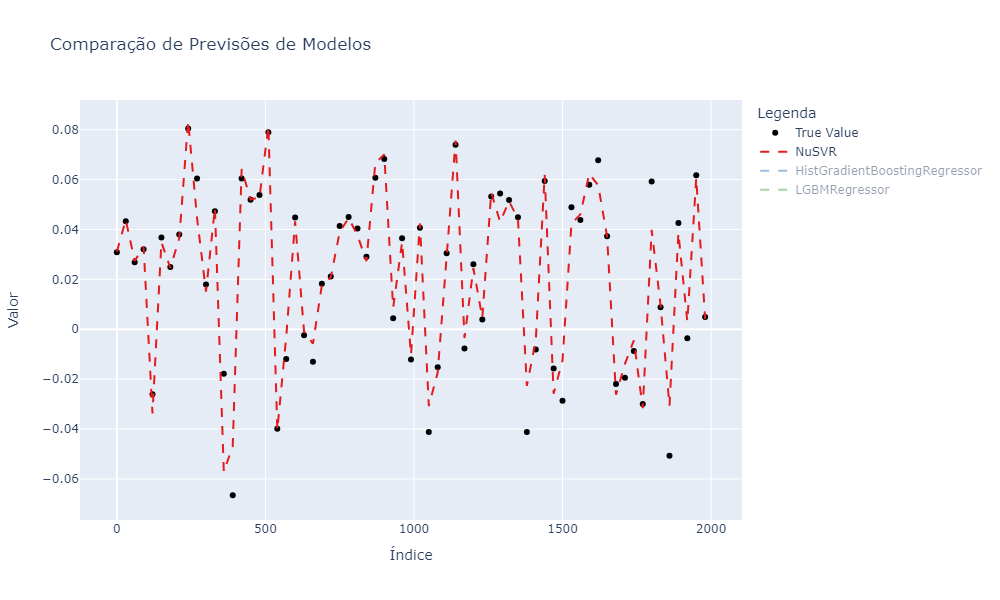
\includegraphics[width=1\linewidth]{NuSVR_Func.png}
        \caption{Função da NuSVR}
    \end{figure}
\end{frame}

\begin{frame}{Função da HistGradientBoostingRegressor}
    \begin{figure}[H]
        \centering
        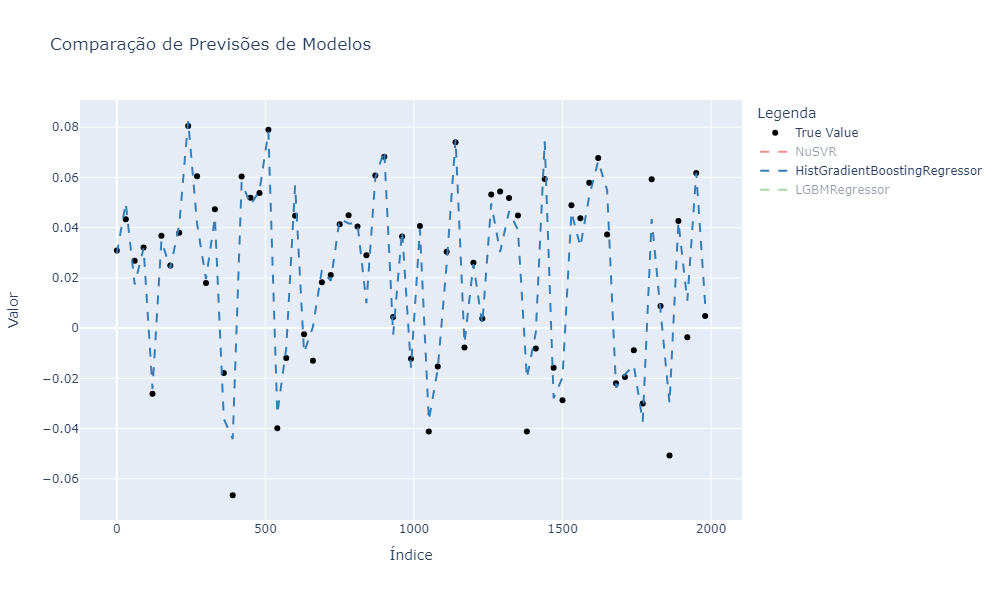
\includegraphics[width=1\linewidth]{HistGradientBoostingRegressor.png}
        \caption{Função da HistGradientBoostingRegressor}
    \end{figure}
\end{frame}

% Slide 13: Discussões sobre Modelos
\begin{frame}{Discussões sobre Modelos}
    \textbf{NuSVR:}
    \begin{itemize}
        \item Maior performance, mas com risco de overfitting ao usar 90\% dos dados como Vetores de Suporte.
    \end{itemize}
    \textbf{LightGBMRegressor:}
    \begin{itemize}
        \item Menor risco de overfitting, melhor capacidade de generalização.
    \end{itemize}
    \textbf{HistGradientBoostingRegressor:}
    \begin{itemize}
        \item Tendência ao sobreajuste, mas com ajustes pode se tornar robusto.
    \end{itemize}
\end{frame}

% Slide 14: Algoritmo Genético - Multivariável
\begin{frame}{Algoritmo Genético: Multivariável}
    \begin{figure}[H]
        \centering
        \includegraphics[width=1\linewidth]{multivariaveis_fitness_grafico.jpg}
        \caption{Gráfico de fitness para AG multivariáveis}
    \end{figure}
    \textbf{Análise:}
    \begin{itemize}
        \item Comportamento esperado do fitness ao longo das gerações.
        \item Possibilidade de overfitting sem cross entropy.
    \end{itemize}
\end{frame}

% Slide 15: Algoritmo Genético - Multivariável (Erros)
\begin{frame}{Algoritmo Genético: Multivariável - Medidas de Erro}
    \begin{figure}[H]
        \centering
        \includegraphics[width=1\linewidth]{multivariaveis_fitness.jpg}
        \caption{Valores de erro do AG de multivariáveis}
    \end{figure}
    \textbf{Análise:}
    \begin{itemize}
        \item Medidas de erro e valores dos parâmetros utilizados.
    \end{itemize}
\end{frame}

% Slide 16: Algoritmo Genético - 80/20
\begin{frame}{Algoritmo Genético: 80/20}
    \begin{figure}[H]
        \centering
        \includegraphics[width=0.8\linewidth]{fitness_80_20.jpg}
        \caption{Gráfico de fitness para AG 80/20}
    \end{figure}
\end{frame}

% Slide 17: Algoritmo Genético - 80/20 (Erros)
\begin{frame}{Algoritmo Genético: 80/20 - Medidas de Erro}
    \begin{itemize}
        \item \textbf{Parâmetros da melhor solução:} [7.93205155e-03, 4.17784195e-04, 6.45921026-03, 1.92005246e-02, -1.96338026e+00, -1.92890651e+00, -1.99986665e+00, -1.93018442e+00, 7.56142420e-02, 6.09533678e-02, -1.87506567e-01, -1.03931572e-01]
        \item \textbf{Fitness da melhor solução:} 0.001500759904008849
        \item \textbf{Index da melhor solução:} 0
        \item \textbf{MAE:} 0.08038562847020014
        \item \textbf{MSE:} 0.010006329160295811
        \item \textbf{RMSE:} 0.10003164079577927
        \item \textbf{MAPE:} 1064.996180354192
    \end{itemize}
\end{frame}
% Slide 19: Conclusão sobre Regressão - Parte 1
\begin{frame}{Conclusão sobre Regressão - Parte 1}
    \textbf{NuSVR:}
    \begin{itemize}
        \item Apresenta bom desempenho, mas é propenso a sobreajuste, comprometendo a generalização.
    \end{itemize}

    \textbf{HistGradientBoostingRegressor:}
    \begin{itemize}
        \item Mostra sinais de sobreajuste, necessitando de ajustes para melhorar sua robustez.
    \end{itemize}
\end{frame}

% Slide 20: Conclusão sobre Regressão - Parte 2
\begin{frame}{Conclusão sobre Regressão - Parte 2}
    \textbf{LightGBMRegressor:}
    \begin{itemize}
        \item Demonstrou maior resistência ao sobreajuste, sendo uma opção mais confiável para ambientes de dados variados.
    \end{itemize}

    \begin{itemize}
        \item MAPE elevado em ambos os métodos, com melhores resultados para o AG multivariável.
    \end{itemize}

\end{frame}

% Slide 18: Conclusões sobre AG
\begin{frame}{Conclusões sobre Algoritmo Genético}
    \begin{itemize}
        \item AG multivariável apresentou melhor desempenho, mas com maior custo computacional.
        \item Aumentar a quantidade de soluções por população melhora o fitness, mas exige mais recursos.
        \item O AG simples rodou para mais equações, mas apresentou desempenho geral pior.
    \end{itemize}
\end{frame}

% Slide 18: Conclusões sobre AG
\begin{frame}{Conclusões Finais}
    \begin{itemize}
        \item Modelo de Escolha: LightGBMRegressor.
        \item Parâmetros: $max\_depth = 10$
    \end{itemize}
    \begin{itemize}
        \item Medidas de Erro:
              \begin{itemize}    \item \textbf{MAE:} 0.0063
                  \item \textbf{MSE:} $69.36$x$10^{-6}$
                  \item \textbf{MAPE:} 313.0708
                  \item \textbf{R²:} 0.9494
              \end{itemize}
    \end{itemize}
\end{frame}


\section{Referências}

\begin{frame}{Referências}

    \begin{footnotesize}
        \begin{thebibliography}{1}

            \bibitem{Arzamasov2018}
            V. Arzamasov, K. Böhm, and P. Jochem, "Towards Concise Models of Grid Stability," in \textit{2018 IEEE International Conference on Communications, Control, and Computing Technologies for Smart Grids (SmartGridComm)}, Aalborg, Denmark, 2018, pp. 1-6, doi: 10.1109/SmartGridComm.2018.8587498.

            \bibitem{SAP2024}
            SAP Insights, "The Smart Grid: How AI is Powering Today’s Energy Technologies," Available: \textit{SAP Insights}, Accessed: Jul. 11, 2024.

            \bibitem{Satu2024}
            Md. Satu and Md. Imran Khan, "Machine Learning Approaches To Predict The Stability of Smart Grid," 2024, doi: 10.21203/rs.3.rs-3866218/v1.

            \bibitem{Shi2024}
            Y. Shi, G. Ke, D. Soukhavong, J. Lamb, Q. Meng, T. Finley, T. Wang, W. Chen, W. Ma, Q. Ye, T. Liu, N. Titov, and D. Cortes, "lightgbm: Light Gradient Boosting Machine," R package version 4.5.0.99, 2024. Available: https://github.com/Microsoft/LightGBM.

            \bibitem{Chen2016}
            T. Chen and C. Guestrin, "XGBoost: A Scalable Tree Boosting System," in \textit{Proceedings of the 22nd ACM SIGKDD International Conference on Knowledge Discovery and Data Mining}, San Francisco, CA, USA, 2016, pp. 785-794, doi: 10.1145/2939672.2939785.

        \end{thebibliography}
    \end{footnotesize}
\end{frame}

\end{document}
